\documentclass[handout]{beamer} % 
%\documentclass{beamer}          
\beamertemplatenavigationsymbolsempty

\usepackage[applemac]{inputenc}
\usepackage{verbatim}
\usepackage{graphicx}
\usepackage{courier}
%\usepackage{pgfpages} 
%\usepackage{handoutWithNotes}
%\pgfpagesuselayout{4 on 1 with notes}[a4paper,border shrink=5mm] 

\usetheme{Warsaw}
\title{Quick review of Git }
\subtitle{R�union de rentr�e 2015}
\author{Pierre Navaro}
\institute{Institut de Math�matique de Rennes}
\date{\today}

\usepackage{xcolor}
\usepackage[procnames]{listings}
\usepackage{textcomp}
\usepackage{setspace}
\usepackage{palatino}
\usepackage{bera}
\usepackage{bbding}
\renewcommand{\lstlistlistingname}{Code Listings}
\renewcommand{\lstlistingname}{Code Listing}
\definecolor{gray}{gray}{0.5}
\definecolor{green}{rgb}{0,0.5,0}
\definecolor{lightgreen}{rgb}{0,0.7,0}
\definecolor{purple}{rgb}{0.5,0,0.5}
\definecolor{darkred}{rgb}{0.5,0,0}
\definecolor{lightblue}{rgb}{0,191,255}

\lstnewenvironment{fortran}[1][]{
 \lstset{language=Fortran,
 basicstyle=\ttfamily\scriptsize\setstretch{1},
 emph={Cf2py},emphstyle=\color{red},
 emph={[3]sqrt,sin,cos,tan},emphstyle={[3]\color{darkred}},
 emph={[4]sll_int32,sll_real64,SLL_ALLOCATE,SLL_ASSERT},emphstyle={[4]\color{purple}\textbf},
 keywordstyle=\color{red}\textbf,
 commentstyle=\color{green}\itshape,
 procnamekeys={subroutine, function},
 procnamestyle=\color{blue}\textbf
}}{}

\lstset{    basicstyle=\ttfamily\bfseries\footnotesize ,     escapeinside={<@}{@>}}
\useinnertheme{circles}
\newenvironment{proenv}{\only{\setbeamercolor{local structure}{fg=green}}}{}
\newenvironment{conenv}{\only{\setbeamercolor{local structure}{fg=red}}}{}

\usepackage{media9}
\usepackage{minted}

\begin{document}

%==============================================================================
\begin{frame}
\titlepage
\end{frame}

\begin{frame}{About Dropbox}
\begin{itemize}[<+->]
\item Dropbox versioning is not free. 
\item Only keep your edits over a period of 30 days. 
\item Privacy and Security ?
\item No differences display.
\item The service have the right to delete information from free and inactive accounts.
\item Users are not allowed to perform encryption.
\end{itemize}
\pause New products based on a git server for collaborating writing.
\begin{itemize}
\item ShareLaTeX \url{https://fr.sharelatex.com}
\item Authorea \url{https://www.authorea.com}
\item Overleaf \url{https://www.overleaf.com}
\end{itemize}
\end{frame}

%==============================================================================

\begin{frame}{About Version Control}
\begin{itemize}[<+->]
\item Records changes to a file or set of files over time.
\item You can recall specific versions later. 
\item You can use it with nearly any type of file on a computer.
\item This is the better way to collaborate on the same document.
\item Every change is committed with an author and a date.
\item Figures are downloaded from Pro Git book : \url{http://git-scm.com/book}.
\item "Become a git guru" tutorial \url{https://www.atlassian.com/git/tutorials/}.
\end{itemize}
\end{frame}

%==============================================================================

\begin{frame}{Local Version Control Systems}
\begin{center}
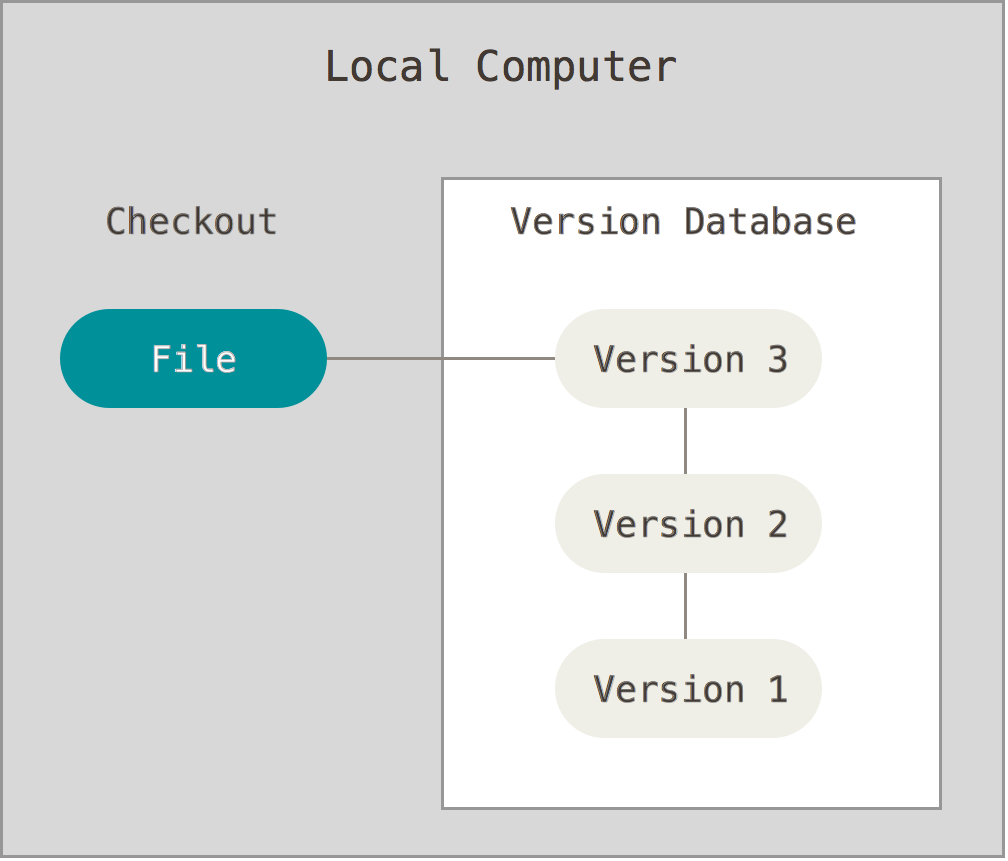
\includegraphics[height=1.8in]{local}
\end{center}
\pause
\begin{itemize}[<+->]
\item One of the most saving popular was a system called RCS
\item[\color{green}\Checkmark]  Available with the Developer Tools with Mac OS X 
\item[\color{red}\XSolidBrush]  Collaboration is not really possible.
\end{itemize}
\end{frame}

%==============================================================================

\begin{frame}{Centralized Version Control Systems}
\begin{center}
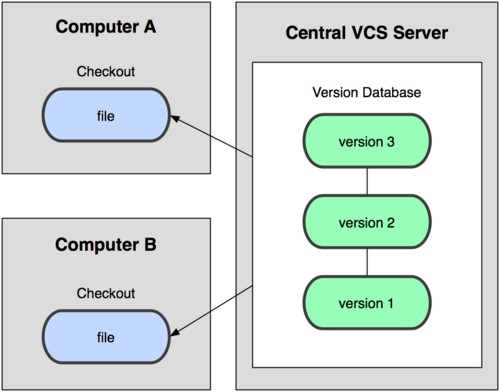
\includegraphics[height=1.5in]{cvs}
\end{center}
\pause
\begin{itemize}[<+->]
\item[\color{green}\Checkmark]   Clients check out files from a central place.
\item[\color{green}\Checkmark]   You know what everyone else on the project is doing
\item[\color{green}\Checkmark]   A single server contains all the versioned files. 
\item[\color{green}\Checkmark]  For many years, this has been the standard (CVS, SVN).
\item[\color{red}\XSolidBrush]  You always need network connection.
\item[\color{red}\XSolidBrush]  If the server is corrupted, with no backup, you lose everything !
\end{itemize}
\end{frame}

%==============================================================================

\begin{frame}{Distributed Version Control Systems}
\begin{center}
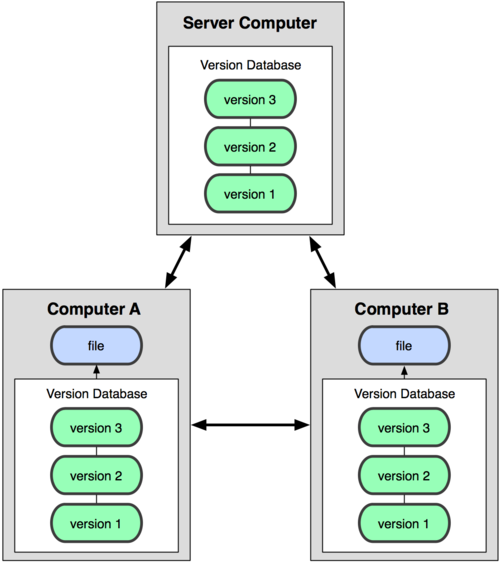
\includegraphics[height=2in]{git}
\end{center}
\pause
\begin{itemize}[<+->]
\item[\color{green}\Checkmark]   Clients fully mirror the repository.
\item[\color{green}\Checkmark]   You can collaborate with different groups of people in different ways simultaneously within the same project.
\item[\color{green}\Checkmark]   No need of network connection.
\item[\color{green}\Checkmark]   Multiple backups.
\end{itemize}
\end{frame}


\begin{frame}[fragile]{Configure Git }
\begin{lstlisting}
$ <@\textcolor{blue}{ git config --global user.name "Pierre Navaro"}@>
\end{lstlisting}\pause\begin{lstlisting}
$ <@\textcolor{blue}{ git config --global user.email "pierre.navaro@univ-rennes1.fr"}@>
\end{lstlisting}\pause\begin{lstlisting}
$ <@\textcolor{blue}{ git config --global core.editor mvim}@>
\end{lstlisting}\pause\begin{lstlisting}
$ <@\textcolor{blue}{ git config --global merge.tool opendiff }@>
\end{lstlisting}
\pause
\begin{lstlisting}
$ <@\textcolor{blue}{ git config --list}@>
user.name=Pierre Navaro
user.email=pierre.navaro@univ-rennes1.fr
core.editor=mvim
merge.tool=opendiff
\end{lstlisting}

Settings are saved on the computer for all your git repositories.
\end{frame}
%==============================================================================
\begin{frame}{Four File status in the repository}
\begin{center}
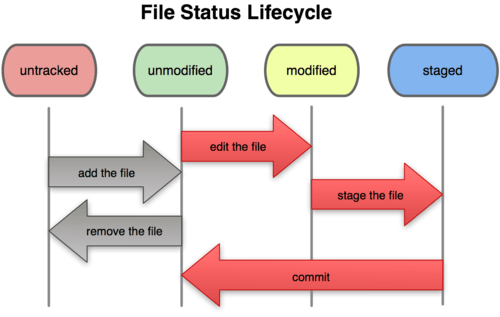
\includegraphics[height=2in]{18333fig0201-tn}
\end{center}
\end{frame}
%==============================================================================

\begin{frame}[fragile]{Initializing a Repository in an Existing Directory }
\begin{lstlisting}
$ <@\textcolor{blue}{ cd article}@>
$ <@\textcolor{blue}{ ls}@>
document.tex	figure.png
\end{lstlisting}\pause\begin{lstlisting}
$ <@\textcolor{blue}{ git init}@>
Initialized empty Git repository in /Users/navaro/article/.git/
\end{lstlisting}\pause\begin{lstlisting}
$ <@\textcolor{blue}{ git status}@>
On branch master
Initial commit
Untracked files:
  (use "git add <file>..." to include in what will be committed)

	document.tex
	figure.png

nothing added to commit but untracked files present 
(use "git add" to track)
\end{lstlisting}
\end{frame}

%==============================================================================

\begin{frame}[fragile]{Adding files in your repository }
\begin{lstlisting}
$ <@\textcolor{blue}{ git add document.tex }@>
$ <@\textcolor{blue}{ git add figure.png}@>
\end{lstlisting}\pause\begin{lstlisting}
$ <@\textcolor{blue}{ git status}@>
On branch master
Initial commit
Changes to be committed:
  (use "git rm --cached <file>..." to unstage)

	new file:   document.tex
	new file:   figure.png
\end{lstlisting}
\pause
\begin{lstlisting}
$ <@\textcolor{blue}{ git commit -m 'Initial project version'}@>
[master (root-commit) 9d23b49] Initial project version
 2 files changed, 0 insertions(+), 0 deletions(-)
 create mode 100644 document.tex
 create mode 100644 figure.png
\end{lstlisting}
\end{frame}

%==============================================================================

\begin{frame}[fragile]{Cloning a New Directory }
\pause
\begin{lstlisting}
$ <@\textcolor{blue}{ git clone git@git.math.cnrs.fr:plm/navaro/projet}@>
Cloning into 'projet'...
Initialized empty Git repository in /git/repositories/plm/navaro/projet.git/
warning: You appear to have cloned an empty repository.
Checking connectivity... done.
\end{lstlisting}
\pause Now you can add and commit your files.
\begin{lstlisting}
$ <@\textcolor{blue}{cd projet/}@>
$ <@\textcolor{blue}{cp ../article/*}@>
$ <@\textcolor{blue}{git add document.tex}@>
$ <@\textcolor{blue}{git add figure.png}@>
$ <@\textcolor{blue}{git commit -m 'Initial version of the project'}@>
\end{lstlisting}\pause \alert{Your files are NOT present on the server!} \pause
\begin{lstlisting}
$ <@\textcolor{blue}{ git status}@>
On branch master
Your branch is based on 'origin/master', but the upstream is gone.
  (use "git branch --unset-upstream" to fixup)
nothing to commit, working directory clean
\end{lstlisting}
\end{frame}

%==============================================================================

\begin{frame}[fragile]{Synchronizing your files on the server }
 By default you are on the "master" branch. 
 \pause
 \begin{lstlisting}
$ <@\textcolor{blue}{ git branch}@>
* master
\end{lstlisting} \pause
Upload your files to the server:
 \pause
\begin{lstlisting}
$ <@\textcolor{blue}{ git push origin master}@>
Counting objects: 3, done.
Delta compression using up to 8 threads.
Compressing objects: 100% (2/2), done.
Writing objects: 100% (3/3), 246 bytes | 0 bytes/s, done.
Total 3 (delta 0), reused 0 (delta 0)
To git@git.math.cnrs.fr:plm/navaro/projet
 * [new branch]      master -> master
\end{lstlisting}
\end{frame}

%==============================================================================
\begin{frame}{Git Workflow}
\begin{center}
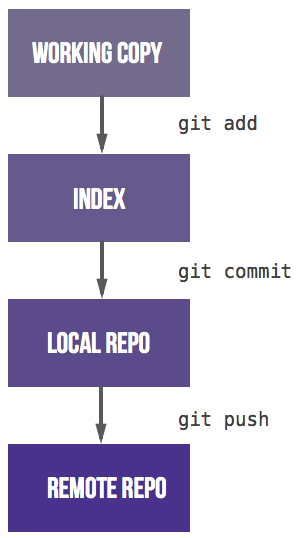
\includegraphics[height=1.8in]{four_stages}
\end{center}
\end{frame}

%==============================================================================

\begin{frame}[fragile]{Cloning an Existing Directory }
Now i change my computer. \pause
\begin{lstlisting}
$ <@\textcolor{blue}{ git clone git@git.math.cnrs.fr:plm/navaro/projet}@>
Cloning into 'projet'...
remote: Counting objects: 3, done.
remote: Compressing objects: 100% (2/2), done.
remote: Total 3 (delta 0), reused 0 (delta 0)
Receiving objects: 100% (3/3), 246 bytes | 0 bytes/s, done.
Checking connectivity... done.
\end{lstlisting}
\pause
\begin{lstlisting}
$ <@\textcolor{blue}{cd projet/}@>
$ <@\textcolor{blue}{ls}@>
document.tex	figure.png
\end{lstlisting}\pause
\begin{lstlisting}
$ <@\textcolor{blue}{ git log}@>
commit 7cef21ac9119ef2fb97065c9e5549550e2f603fd
Author: Pierre Navaro <pierre.navaro@univ-rennes1.fr>
Date:   Fri Oct 2 13:51:43 2015 +0200

    Initial version of the project
\end{lstlisting}
\end{frame}

%==============================================================================

\begin{frame}[fragile]{Display and Create a Branch }
Display all branches :
\begin{lstlisting}
$ <@\textcolor{blue}{ git branch -a}@>
* master
  remotes/origin/HEAD -> origin/master
  remotes/origin/master
\end{lstlisting}
\pause Create your own branch and switch:
\begin{lstlisting}
$ <@\textcolor{blue}{ git branch pierre-branch}@>
$ <@\textcolor{blue}{ git checkout pierre-branch}@>
\end{lstlisting}\pause
\begin{lstlisting}
Switched to branch 'pierre-branch'
\end{lstlisting}
\pause Check
\begin{lstlisting}
$ <@\textcolor{blue}{ git branch}@>
  master
* pierre-branch
\end{lstlisting}
\alert{Files could be different or non existant between branches but are at the same place on the file system}
\end{frame}


%==============================================================================

\begin{frame}[fragile]{Contributing }
Modify the file document.tex \pause
\begin{lstlisting}
$ <@\textcolor{blue}{ git status}@>
On branch pierre-branch
Changes not staged for commit:
  (use "git add <file>..." to update what will be committed)
  (use "git checkout -- <file>..." to discard changes in working directory)
	modified:   document.tex
no changes added to commit (use "git add" and/or "git commit -a")
\end{lstlisting}\pause\begin{lstlisting}
$ <@\textcolor{blue}{ git diff}@>
diff --git a/document.tex b/document.tex
index a608114..e69de29 100644
--- a/document.tex
+++ b/document.tex
@@ -1,3 +0,0 @@
-Exemple Git pour la journ�e de rentr�e
\end{lstlisting}
\end{frame}

\begin{frame}[fragile]{Locally saving your modifications}
\pause
\begin{lstlisting}
$ <@\textcolor{blue}{ git add document.tex}@>
 \end{lstlisting}
\pause Checking which files are ready to be committed.
\begin{lstlisting}
$ <@\textcolor{blue}{ git status}@>
On branch pierre-branch
Changes to be committed:
  (use "git reset HEAD <file>..." to unstage)
	modified:   document.tex
\end{lstlisting}
\pause Now save your work on the local branch.
\begin{lstlisting}
$ <@\textcolor{blue}{ git commit -m 'Some modification is available'}@>
[pierre-branch 8c6bf81] Some modification is available
 1 file changed, 3 insertions(+)
\end{lstlisting}

\end{frame}

%==============================================================================

\begin{frame}[fragile]{Fast commit}

\begin{center}
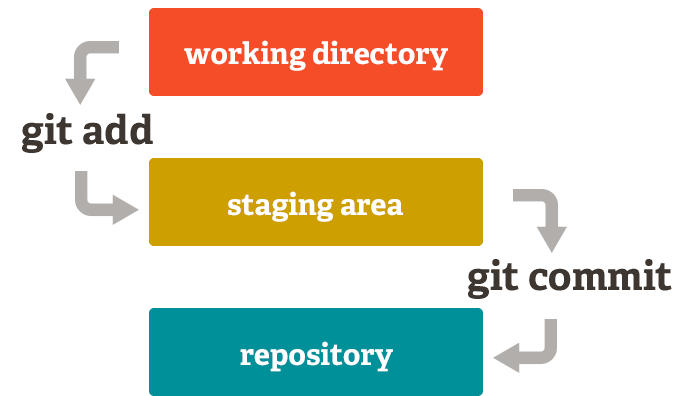
\includegraphics[height=1.2in]{index1}
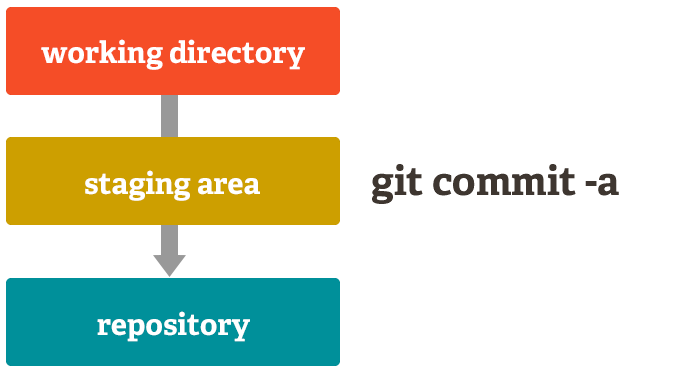
\includegraphics[height=1.2in]{index2}
\end{center}
\alert{Use it carefully!}

\pause How to share your work and make it available on the server?

\end{frame}

%==============================================================================

\begin{frame}[fragile]{Option 1 : Merge to the main branch and push}
\begin{lstlisting}
$ <@\textcolor{blue}{ git checkout master }@>
Switched to branch 'master'
Your branch is up-to-date with 'origin/master'.
\end{lstlisting}\pause\begin{lstlisting}
$ <@\textcolor{blue}{ git merge pierre-branch }@>
Updating 7cef21a..8c6bf81
Fast-forward
 document.tex | 3 +++
 1 file changed, 3 insertions(+)
 \end{lstlisting}\pause\begin{lstlisting}
$ <@\textcolor{blue}{ git push origin master }@>
Counting objects: 3, done.
Delta compression using up to 8 threads.
Compressing objects: 100% (3/3), done.
Writing objects: 100% (3/3), 351 bytes | 0 bytes/s, done.
Total 3 (delta 0), reused 0 (delta 0)
To git@git.math.cnrs.fr:plm/navaro/projet
   7cef21a..8c6bf81  master -> master
\end{lstlisting}
\end{frame}

%==============================================================================

\begin{frame}[fragile]{ Option 2 : Push your branch to the server}
\begin{lstlisting}
$ <@\textcolor{blue}{ git checkout pierre-branch }@>
Switched to branch 'pierre-branch'
 \end{lstlisting}\pause\begin{lstlisting}
$ <@\textcolor{blue}{git push origin pierre-branch }@>
Total 0 (delta 0), reused 0 (delta 0)
To git@git.math.cnrs.fr:plm/navaro/projet
 * [new branch]      pierre-branch -> pierre-branch
\end{lstlisting}
\pause
\begin{lstlisting}
$ <@\textcolor{blue}{ git branch -a}@>
  master
* pierre-branch
  remotes/origin/HEAD -> origin/master
  remotes/origin/master
  remotes/origin/pierre-branch
\end{lstlisting}
\end{frame}

%==============================================================================
 
\begin{frame}[fragile]{Updating from the Repository}
The master branch has changed. To get all new updates :
\pause
\begin{lstlisting}
$ <@\textcolor{blue}{ git checkout master }@>       (change to master)
Switched to branch 'master'
\end{lstlisting}\pause\begin{lstlisting}
$ <@\textcolor{blue}{ git fetch origin  }@>         (download changes from repository)
\end{lstlisting}\pause\begin{lstlisting}
$ <@\textcolor{blue}{ git merge origin/master }@>   (update local branch master)
\end{lstlisting}\pause\begin{lstlisting}
$ <@\textcolor{blue}{ git checkout pierre-branch }@>(back to your branch)
Switched to branch 'pierre-branch'
\end{lstlisting}\pause\begin{lstlisting}
$ <@\textcolor{blue}{ git merge master }@>          (update your branch)
 \end{lstlisting}
\pause If you have conflict, no problem just do :
\begin{lstlisting}
$ <@\textcolor{blue}{ git mergetool}@>
 \end{lstlisting}
A nice editor helps you to choose the right version. Close and :
\begin{lstlisting}
$ <@\textcolor{blue}{ git commit -m 'Update and fixed conflicts'}@>
\end{lstlisting}
\end{frame}

%==============================================================================
\begin{frame}{Git cycle on a single branch}
\begin{center}
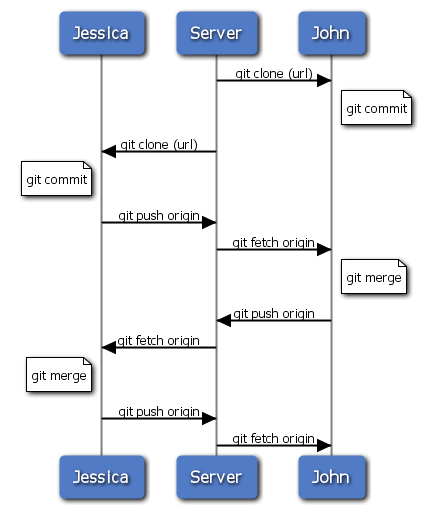
\includegraphics[height=2.5in]{git_cycle}
\end{center}
\end{frame}



%==============================================================================
\begin{frame}{Progressive-stability branching}
\begin{center}
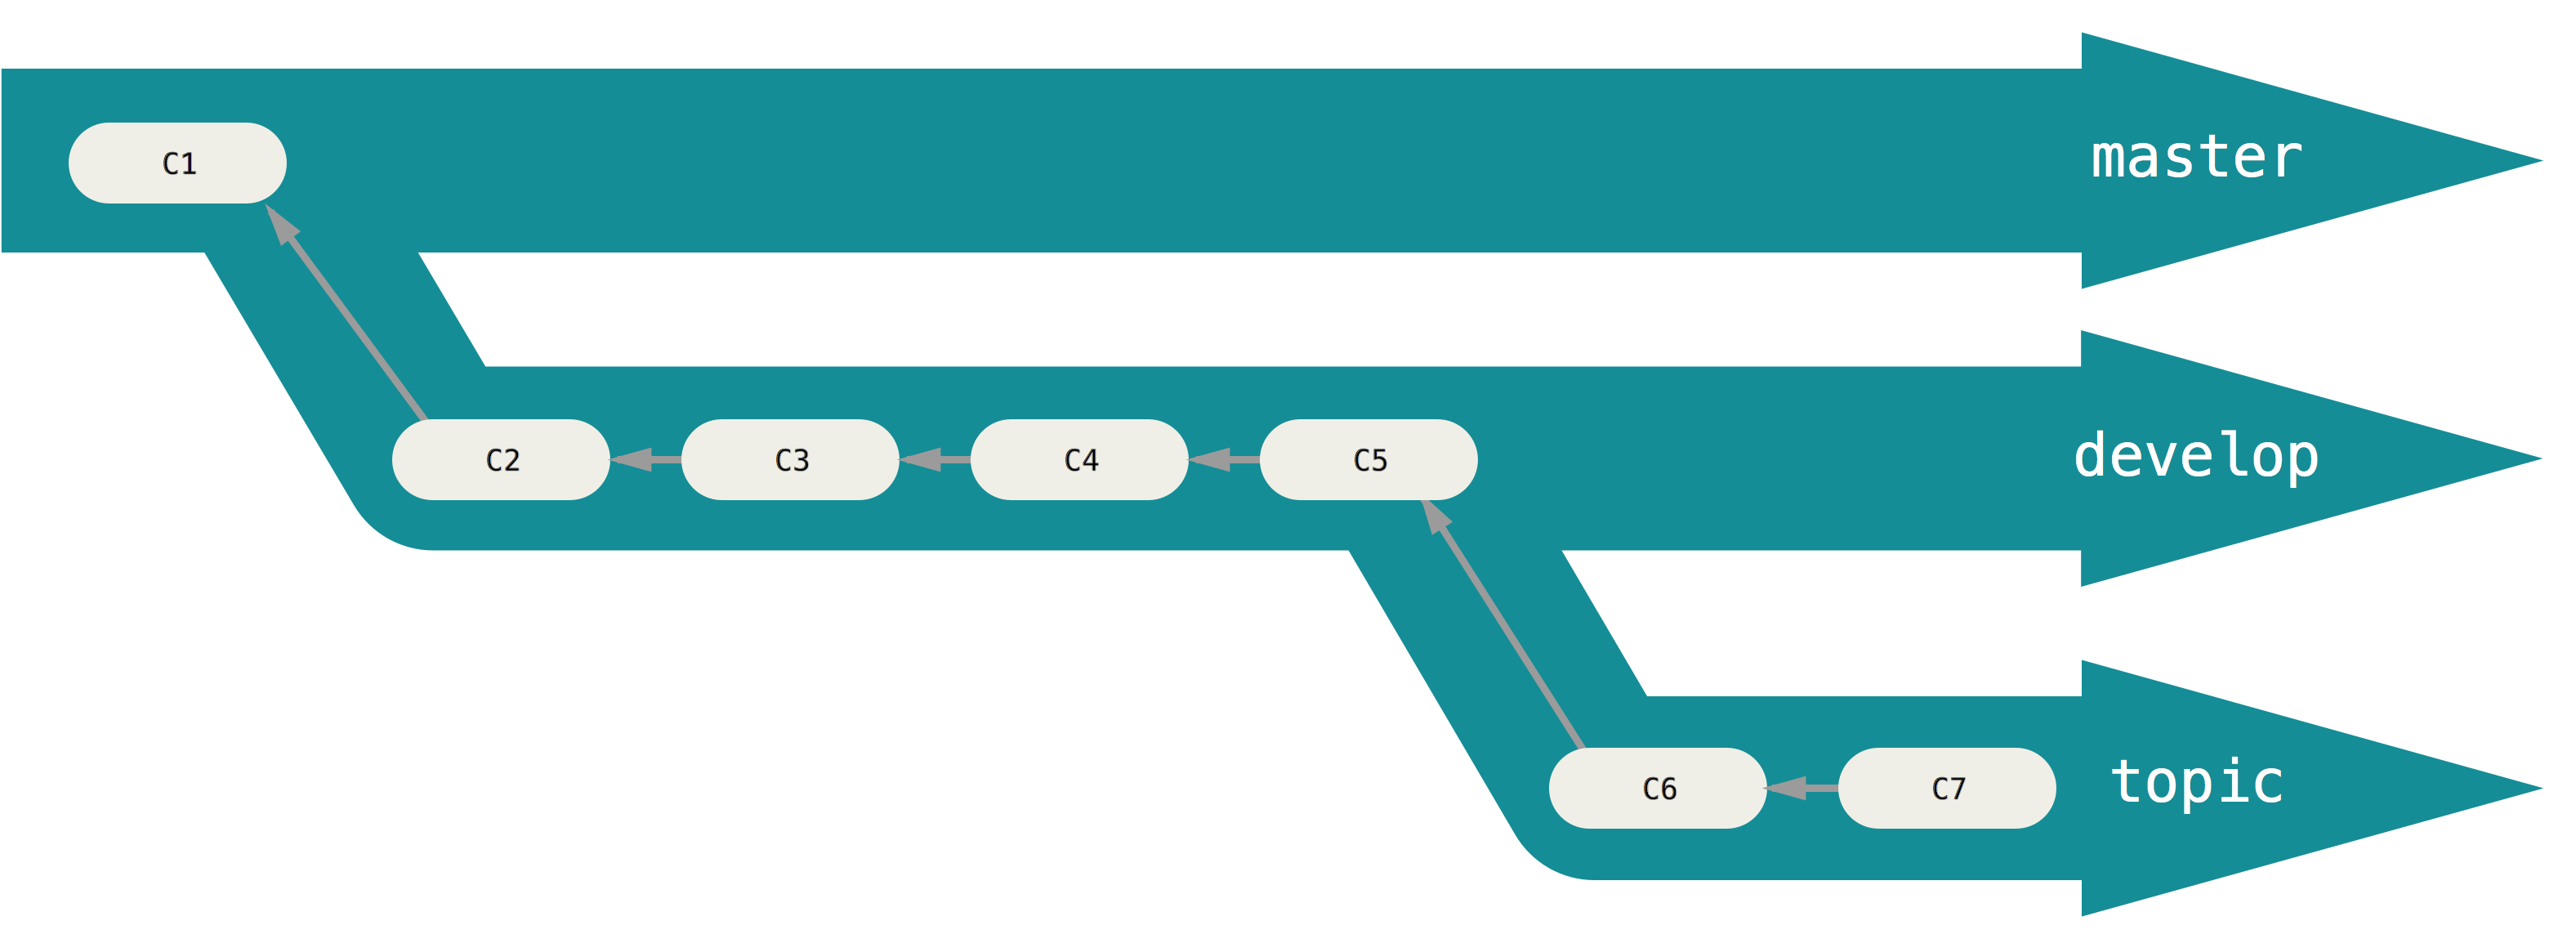
\includegraphics[height=1.5in]{lr-branches-2}
\end{center}
\end{frame}

%==============================================================================
\begin{frame}{GitHub Desktop - Modifications view}
\begin{center}
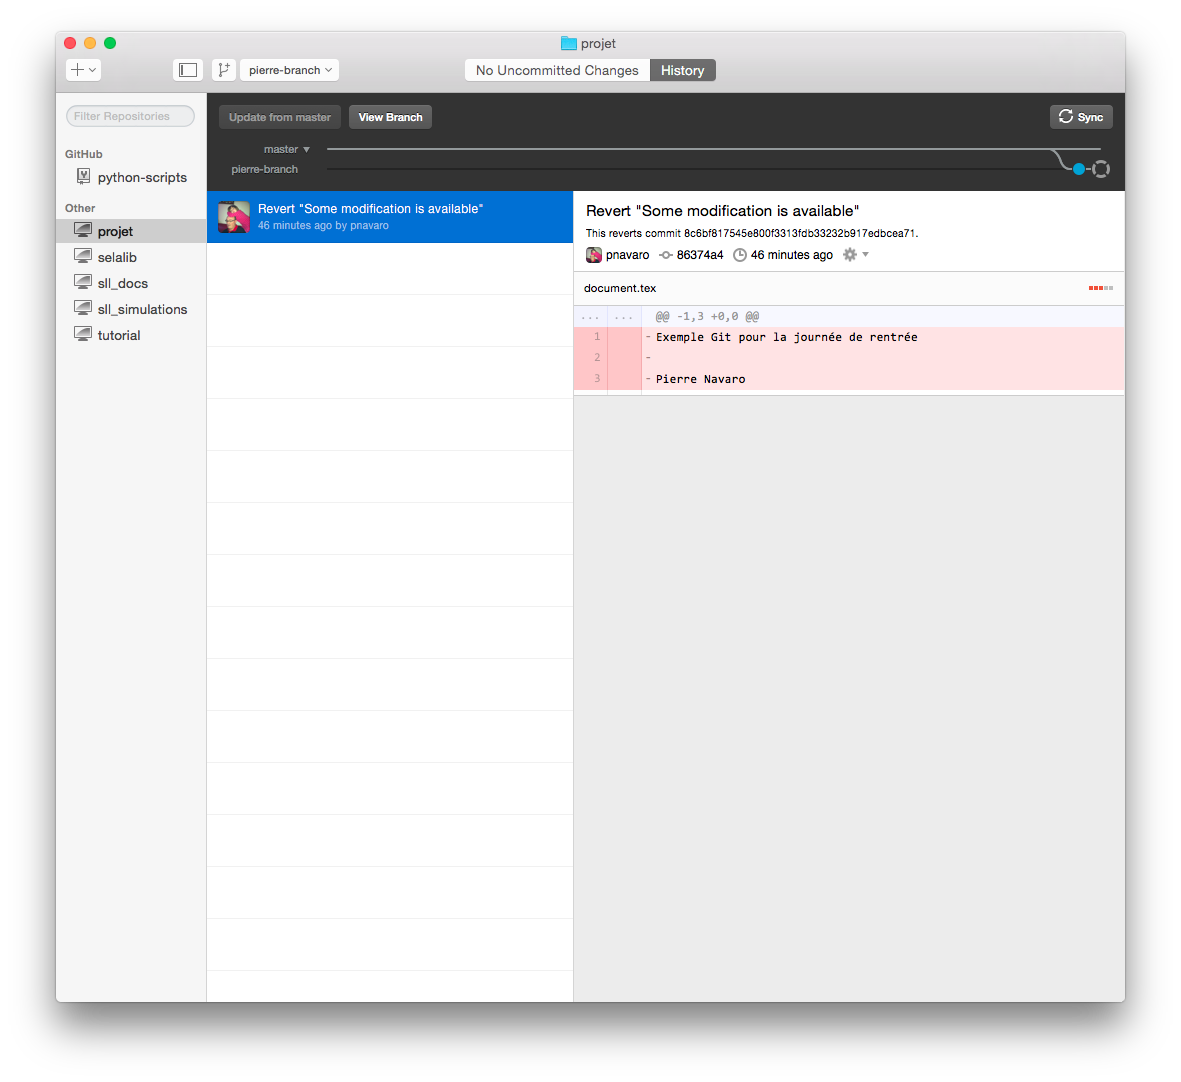
\includegraphics[height=3.in]{desktop}
\end{center}
\end{frame}

%==============================================================================
\begin{frame}{GitHub Desktop - History view}
\begin{center}
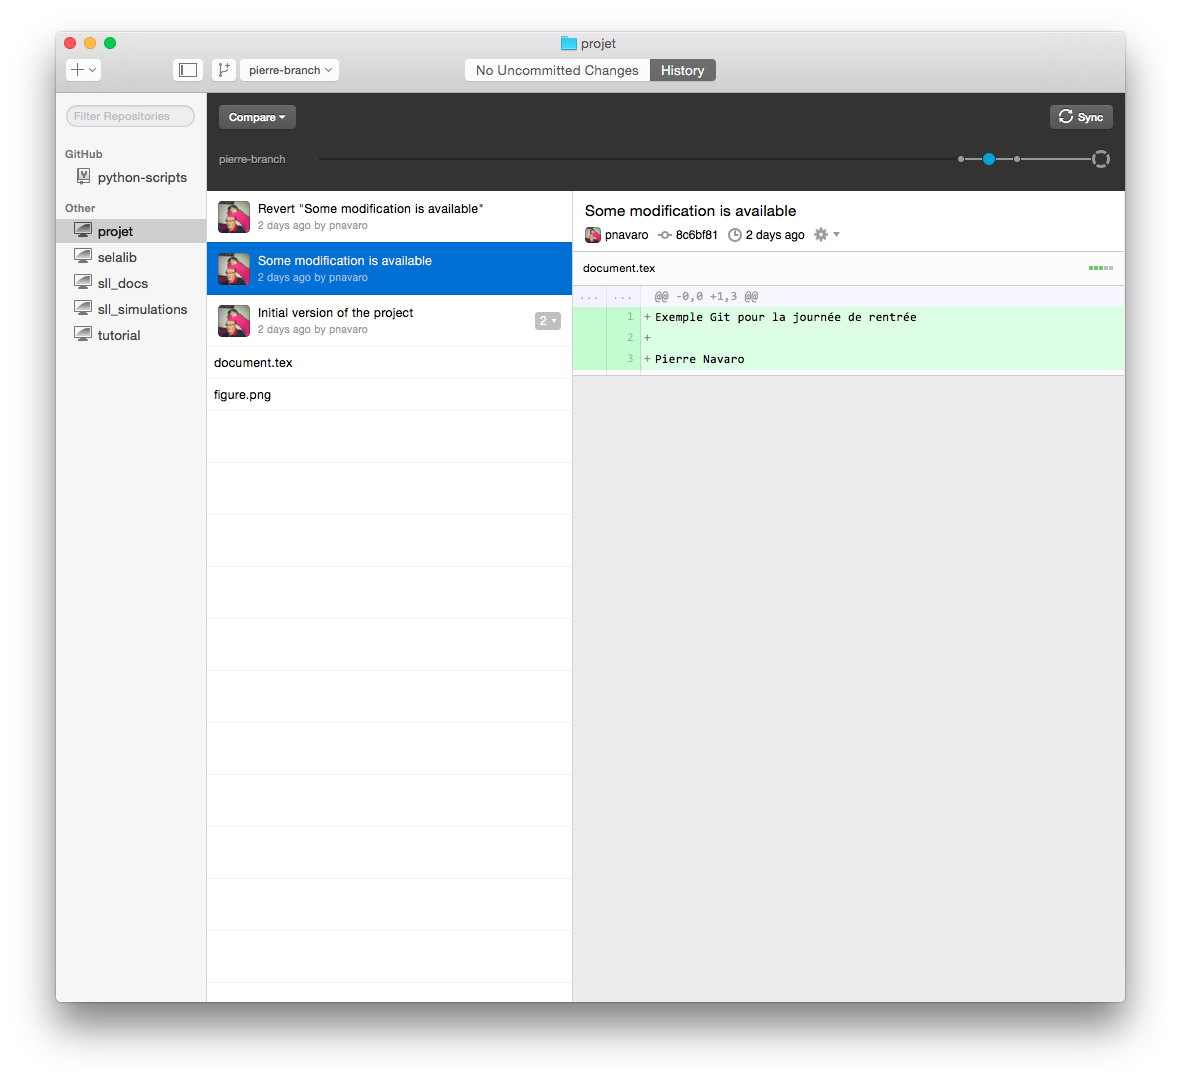
\includegraphics[height=3.in]{desktop2}
\end{center}
\end{frame}

%==============================================================================
\begin{frame}{Why Git?}
Tracking and controlling changes in the software.
\begin{itemize}[<+->]
\item[\color{green}\Checkmark] Branches : Frictionless Context Switching, Role-Based Codelines. 
\item[\color{green}\Checkmark] Everything is local : Git is fast.
\item[\color{green}\Checkmark] Multiple Backups.
\item[\color{green}\Checkmark] It's impossible to get anything out of Git other than the exact bits you put in.
\item[\color{green}\Checkmark] Staging Area : intermediate index between working directory and repository.
\item[\color{red}\XSolidBrush]  Sometimes confusing for new users.
\end{itemize}
\pause Some tips.
\begin{itemize}
\item Install bash-completion and source git-prompt.sh.
\item use GitHub Desktop \url{https://desktop.github.com/}
\end{itemize}
\end{frame}



\end{document}

